\documentclass[10 pt]{report} % Par défaut, la taille de la police est de 10
% PACKAGES IMPORTS
\usepackage[utf8]{inputenc} % Pour dire que le format d'écriture sera UTF-8
\usepackage[french]{babel} % Pour changer la langue
\usepackage{color} % Pour les couleurs
\usepackage{hyperref} % Pour ajouter des liens
\usepackage{amsmath,amsfonts,amssymb} % Pour les symboles mathématiques
\usepackage{graphicx} % Pour insérer les figures
\usepackage{minted} % Pour insérer du code
\usepackage[    % Pour la bibliographie
    backend=biber,
    style=ieee,
    citestyle=ieee
  ]{biblatex}
\addbibresource{biblio.bib}

\title{Mon arrivée en M1 Bioinfo à Bordeaux}
\author{Bobby le bioinformaticien}
\date{Octobre 2020}


\begin{document}

% PAGE DE GARDE
\maketitle

\renewcommand{\contentsname}{Sommaire}
\tableofcontents
\thispagestyle{empty}


\newpage
\setcounter{page}{1}
\chapter{Les Cours en M1}
    \section{ANGLAIS}
    
        {\Huge Sujet de l'oral d'\textsc{Anglais}}\\
        \noindent Vous devrez trouver une \underline{application mobile} ayant un lien avec la \textcolor{red}{bioinformatique}. Un diaporama sera a présenter devant les autres étudiants expliquant l'application choisie. Durée : \textbf{10 min. d'oral + 5 min. de questions}.\\ 
        \indent Un résumé devra aussi être \textit{rendu la veille} de votre oral à l'adresse : \href{mailto:oral-anglais@u-bdx.fr}{oral-anglais@u-bdx.fr}. Vous nommerez le fichier de cette manière : \\ \texttt{NOM\_Prenom\_NomDeLApplication.pdf}.

    \section{BIOSTATS}
        Loi de la gravitation de Newton :
        \begin{math}
            F=G \dfrac{m_1 m_2}{d^2}
        \end{math}
    
    \section{IMAJS}
        Dans ce cours, l'utilisation du logiciel ImageJ a une grande importance. Il permet de modifer des images en améliorant la netteté ou bien au contraire ajouter du bruit (\textsc{Figure}~\ref{fig:clown}).
        
        \begin{figure}[h]
            \centering
            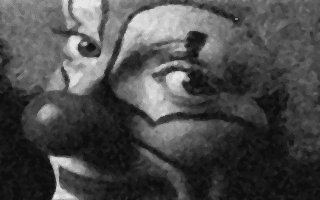
\includegraphics[scale=0.4]{clown_Noise-gaussian_Filter_Median-1-3fois.png}
            \caption{Image ayant subit un bruit gaussien à l'aide d'ImageJ}
            \label{fig:clown}
        \end{figure}
        
        
        
    \section{OBI}

        To estimate the true substitutions number, we calculate the Hamming distance between the initial sequence and the mutate sequence created. For that, we have used the definition of the distance between two string given by R. Hamming \cite{hamming_error_1950}. While comparing two strings of equal length, Hamming distance is the number of positions in which the two nucleotides are different.\\
    \section{APU}
        \subsection{USI}
            Un cours où on apprend à utiliser Linux mais pas que. Bash est notre meilleur ami.
        \subsection{Programmation}
            Python le fameux serpent !
            \inputminted{python}{hamming_function.py}
        \subsection{Algo}
            Les piles, les files vous verrez. LILO and FILO in english.
    
    
    
\chapter{Bordeaux}
    \section{Une ville sympa}
        Bordeaux est une commune du Sud-Ouest de la France. Capitale de la Gaule aquitaine sous l'Empire romain pendant près de 200 ans ; puis du Duché d'Aquitaine, de la province royale de Guyenne et du siècle des lumières, elle est aujourd'hui le chef-lieu et la préfecture de la région Nouvelle-Aquitaine, du département de la Gironde et le siège de Bordeaux Métropole.\\ Source : Wikipédia.
        
    \section{Pleins d'activités}
        \begin{itemize}
            \item Plonger dans le Bordeaux médiéval en visitant la Grosse Cloche et la Porte Cailhau
            \item Admirer les reflets de la ville sur le Miroir d’eau
            \item Profiter d’une vue panoramique sur tout Bordeaux en montant au sommet de la Flèche Saint Michel ou de la Tour Pey Berland
            \item Faire une pause nature au Jardin Public rive gauche ou au Jardin Botanique rive droite
            \item Découvrir la crypte, les sarcophages et la basilique du site archéologique de Saint Seurin
            \item Visiter les salons de l’Hôtel de Ville
            \item Faire le tour des « Marchés ronds » de la ville : le Marché de Lerme et la Halle des Chartrons (réalisés par l’architecte municipal Charles Burguet) et l’élégant Marché des Grands Hommes
            \item Se croire à Rome en admirant l’amphithéâtre antique du Palais Gallien
            \item Visiter Darwin, friche militaire réhabilitée en lieu cool avec skate parc, épicerie bio et restaurant stylé
            \item Lever les yeux et repérer les mascarons typiques de la ville… plus de 3000 différents !
            \item Louer un Vcub et faire la boucle des quais (6.7 km) en passant par les deux ponts emblématiques : le Pont de Pierre et le Pont Chaban-Delmas
        \end{itemize}
\chapter{L'AMBB}
    \section{Une asso super}
    
        Une asso vraiment top et un bureau génial (\textsc{Table}~\ref{tab:ambb}).
        
        \begin{table}[h]
        \centering
        \caption{Tableau récapitulatif des membres du Bureau 2019/2020 de l'AMBB}
        
        \begin{tabular}{|c|c|c|}
                \hline
                Nom     & Prénom    & Fonction   \\ \hline
                BOLTEAU & Mathieu   & Président  \\ \hline
                ALVES   & Marine    & Secrétaire \\ \hline
                PETRUS  & Louis     & Trésorier  \\ \hline
                CARRIAT  & Mélanie   & VP Com     \\ \hline
                LESOURD & Valentine & VP Event   \\ \hline
            \end{tabular}
            \label{tab:ambb}
        \end{table}

\newpage
\addcontentsline{toc}{chapter}{Bibliographie} % Ajoute la biblio au sommaire
\printbibliography
\end{document}
